\documentclass{article}
\usepackage[utf8]{inputenc}
\usepackage[T2A]{fontenc}
\usepackage[english,russian]{babel}
\usepackage[left=1.5cm,right=1.5cm,top=2cm,bottom=2cm]{geometry}
\usepackage{hyperref}
\usepackage{enumitem}
\usepackage{graphicx} %библиотека для графики и картинок
\DeclareGraphicsExtensions{.pdf,.png,.jpg}
\usepackage{listings}


\begin{document}
% НАЧАЛО ТИТУЛЬНОГО ЛИСТА
\begin{center}
    \Large
    Федеральное государственное автономное \\
    образовательное учреждение высшего образования \\ 
    «Национальный исследовательский университет ИТМО»\\
    \vspace{0.5cm}
    \large
    
    \vspace{1cm}
    \Large
    \textbf{По дисциплине «Информационная безопасность»} \\
        Лабораторная работа №7\\
        Безопасность браузера и анализ сетевого
трафика
    \large
    \vspace{8cm}

    \begin{minipage}{.33\textwidth}
    \end{minipage}
    \hfill
    \begin{minipage}{.4\textwidth}
    
        \textbf{Студент}: \vspace{.1cm} \\
        \ Дениченко Александр Олегович P3412\\
        \textbf{Практик}:  \\
        \ Маркина Татьяна Анатольевна
    \end{minipage}
    \vfill
Санкт-Петербург\\ 2025 г.
\end{center}
\pagestyle{empty}
% КОНЕЦ ТИТУЛЬНОГО ЛИСТА 
\newpage
\pagestyle{plain}

\section*{Цель}
Изучить настройки безопасности браузера и понять, какие данные передаются между
браузером и сайтом.

\section{Настройка браузера}





\section*{Результаты}


\end{document}

\begin{center}
  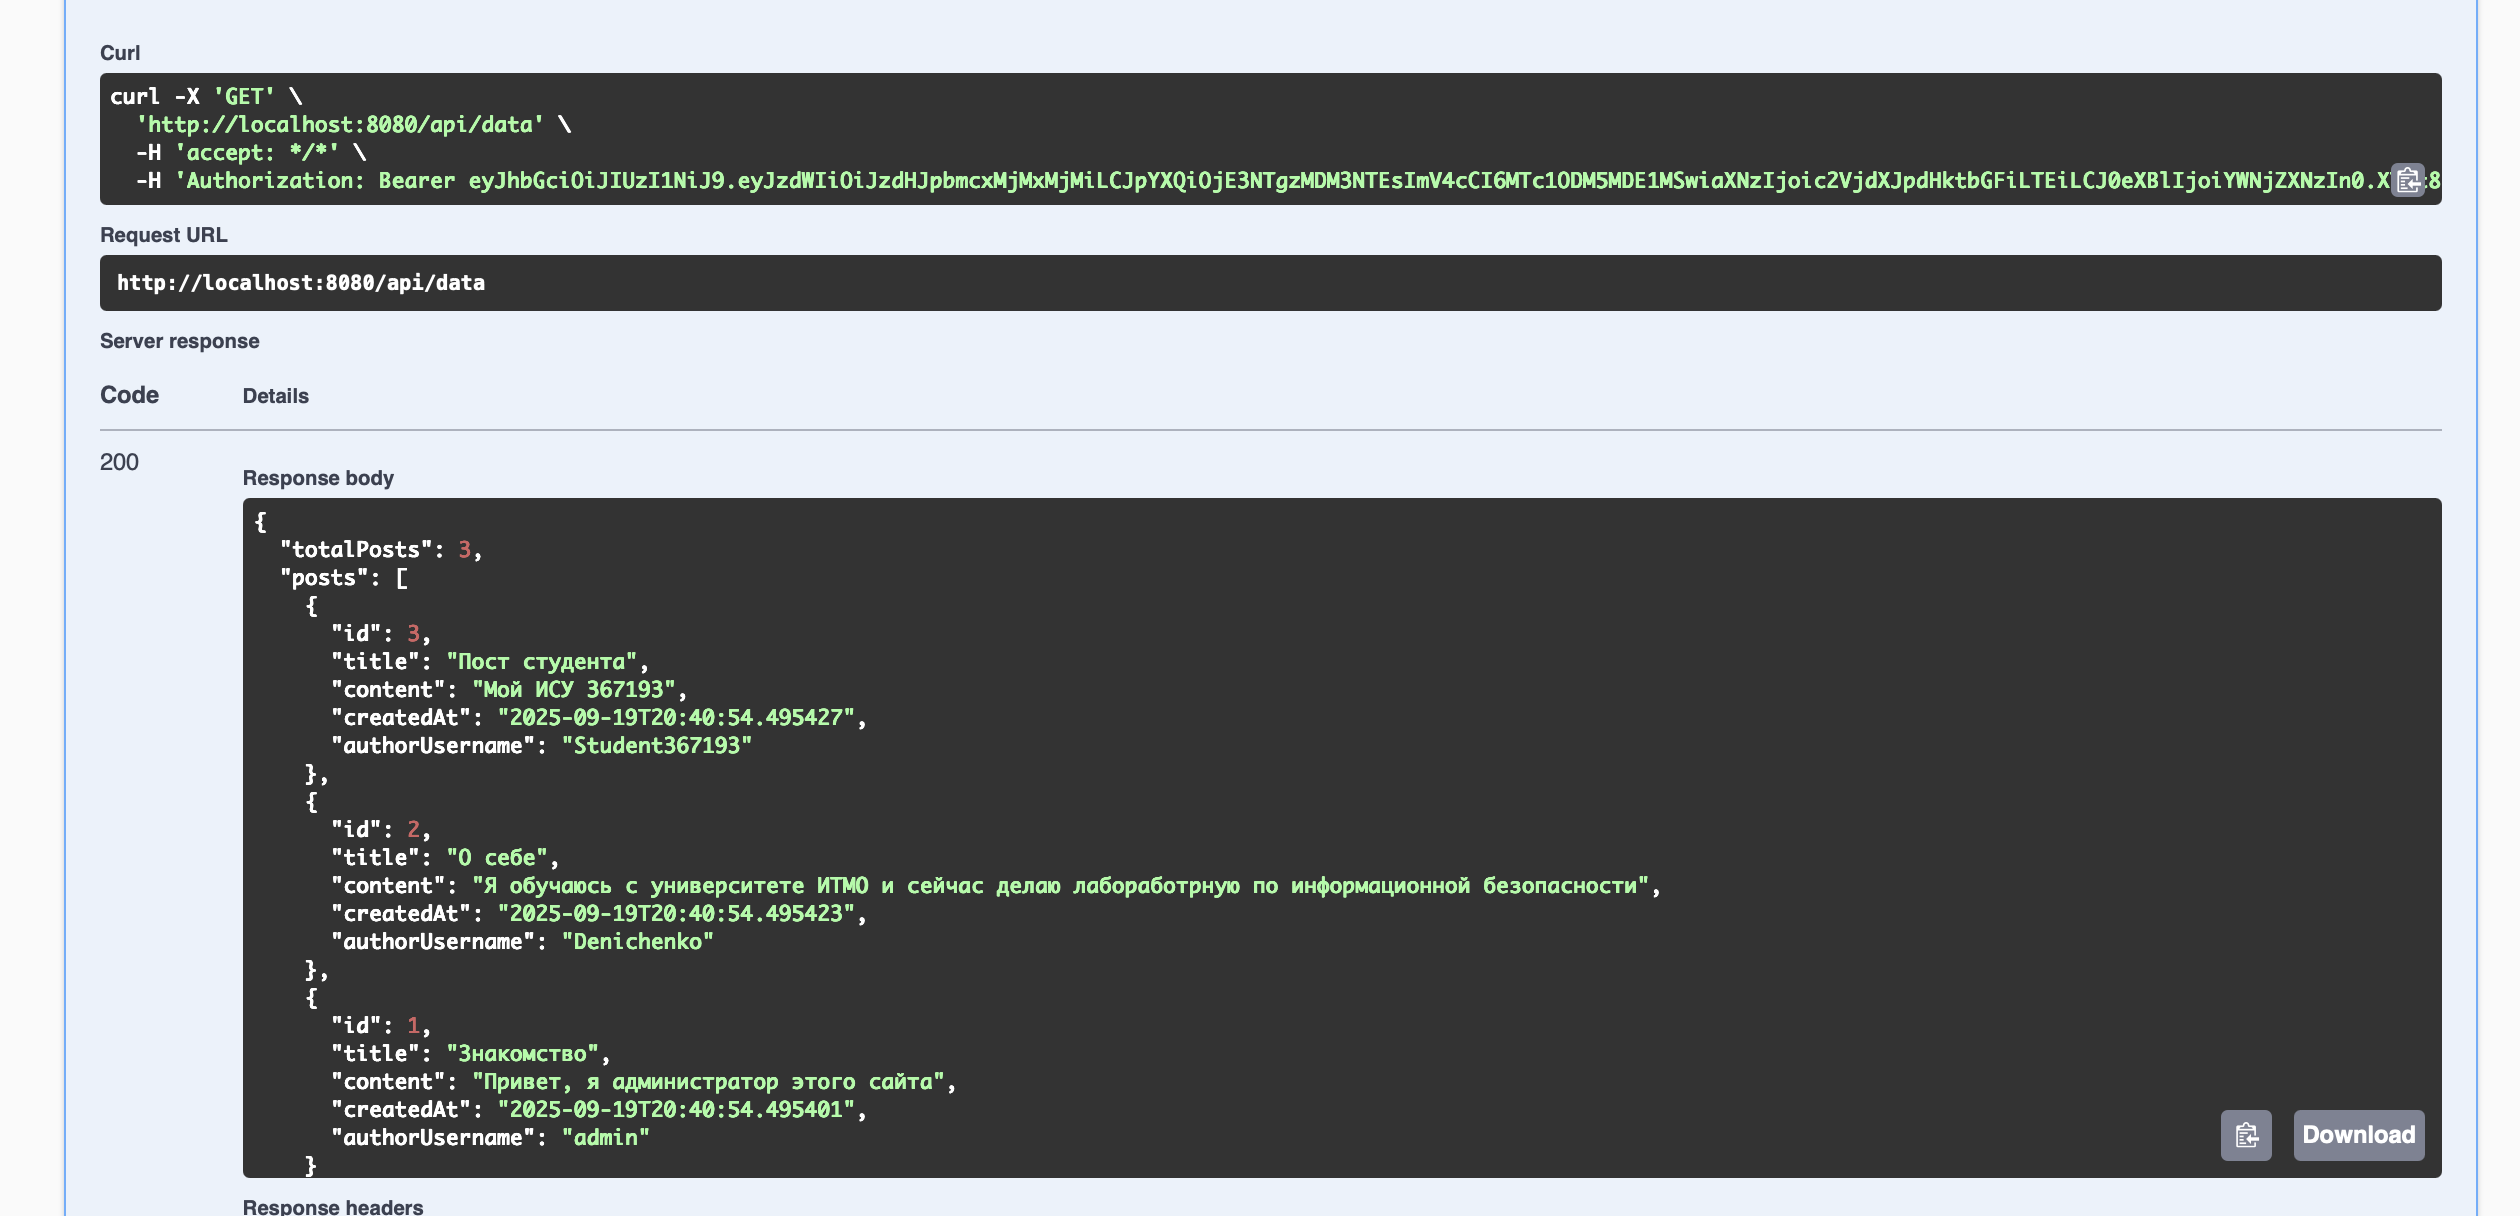
\includegraphics[width=.9\textwidth]{posts}
\end{center}

\href{https://github.com/Alex-de-bug/security-lab-1/actions/runs/17864752066}{Последний верный CI} (https://github.com/Alex-de-bug/security-lab-1/actions/runs/17864752066)

\begin{lstlisting}
  </div><script>alert(1);</script><div>
\end{lstlisting}